% ==============================================================================
% Sustentación: Tubería CNN en OpenACC (Reto 1)
% Maestría en Ciencias de la Información y las Comunicaciones (MCIC)
% Universidad Distrital Francisco José de Caldas
% ==============================================================================
\documentclass[aspectratio=169,10pt]{beamer}

\usepackage{fontspec}
\usepackage{graphicx}
\usepackage{tikz}
\usepackage{xcolor}
\usepackage{booktabs}
\usepackage{array}
\usepackage{amsmath}
\usetikzlibrary{calc,positioning,shapes.geometric,arrows.meta,shadows,fit}

% % Tipografía Institucional Oficial (Manual de Identidad Institucional UD, Pág. 15)
% 1. Cambria: Tipografía básica institucional para logosímbolo, títulos y dependencias
\newfontfamily\cambriafont{cambria.ttc}[
  Path = assets/fonts/,
  BoldFont = cambriab.ttf,
  ItalicFont = cambriai.ttf,
  BoldItalicFont = cambriaz.ttf
]

% 2. Times New Roman: Tipografía complementaria para cuerpo de texto y documentos
\setsansfont{times.ttf}[
  Path = assets/fonts/,
  BoldFont = timesbd.ttf,
  ItalicFont = timesi.ttf,
  BoldItalicFont = timesbi.ttf
]
\setmainfont{times.ttf}[
  Path = assets/fonts/,
  BoldFont = timesbd.ttf,
  ItalicFont = timesi.ttf,
  BoldItalicFont = timesbi.ttf
]

% Paleta de colores oficial (Manual de Identidad Institucional UD)
\definecolor{UDRed}{HTML}{ED3237}       % Rojo gules institucional
\definecolor{UDDarkRed}{HTML}{B71C1C}   % Rojo oscuro contraste
\definecolor{UDGold}{HTML}{B49739}      % Dorado oro
\definecolor{UDBlue}{HTML}{1291C0}      % Azul azur
\definecolor{UDGreen}{HTML}{00A859}     % Verde sinople
\definecolor{UDDarkGreen}{HTML}{047857} % Verde oscuro
\definecolor{UDSilver}{HTML}{64748B}    % Gris pizarra
\definecolor{UDSable}{HTML}{1E293B}     % Carbón oscuro (alta legibilidad)
\definecolor{UDLightGray}{HTML}{F8FAFC} % Fondo de tarjetas
\definecolor{UDBorder}{HTML}{CBD5E1}    % Borde suave

% Configuración de márgenes en Beamer (3.15cm para librar la franja roja izquierda)
\setbeamertemplate{navigation symbols}{}
\setbeamersize{text margin left=3.15cm, text margin right=0.75cm}

% Estilo general de colores
\setbeamercolor{normal text}{fg=UDSable}

% Estilo de títulos de diapositivas con tipografía oficial Cambria
\setbeamertemplate{frametitle}{
  \vspace{0.45cm}
  \begin{minipage}{\textwidth}
    {\cambriafont\fontsize{13pt}{15pt}\bfseries\color{UDSable}\insertframetitle\par}
    \ifx\insertframesubtitle\@empty\else
      \vskip2pt
      {\cambriafont\fontsize{8pt}{10pt}\bfseries\color{UDRed}\insertframesubtitle\par}
    \fi
  \end{minipage}
}

% Pie de página con numeración
\setbeamertemplate{footline}{
  \ifnum\thepage>1
    \hfill{\color{UDSilver}\fontsize{7pt}{8pt}\selectfont \insertframenumber\,/\,\inserttotalframenumber}\hspace{0.75cm}\vspace{0.35cm}
  \fi
}

% Fondo por defecto para diapositivas de contenido
\setbeamertemplate{background}{
  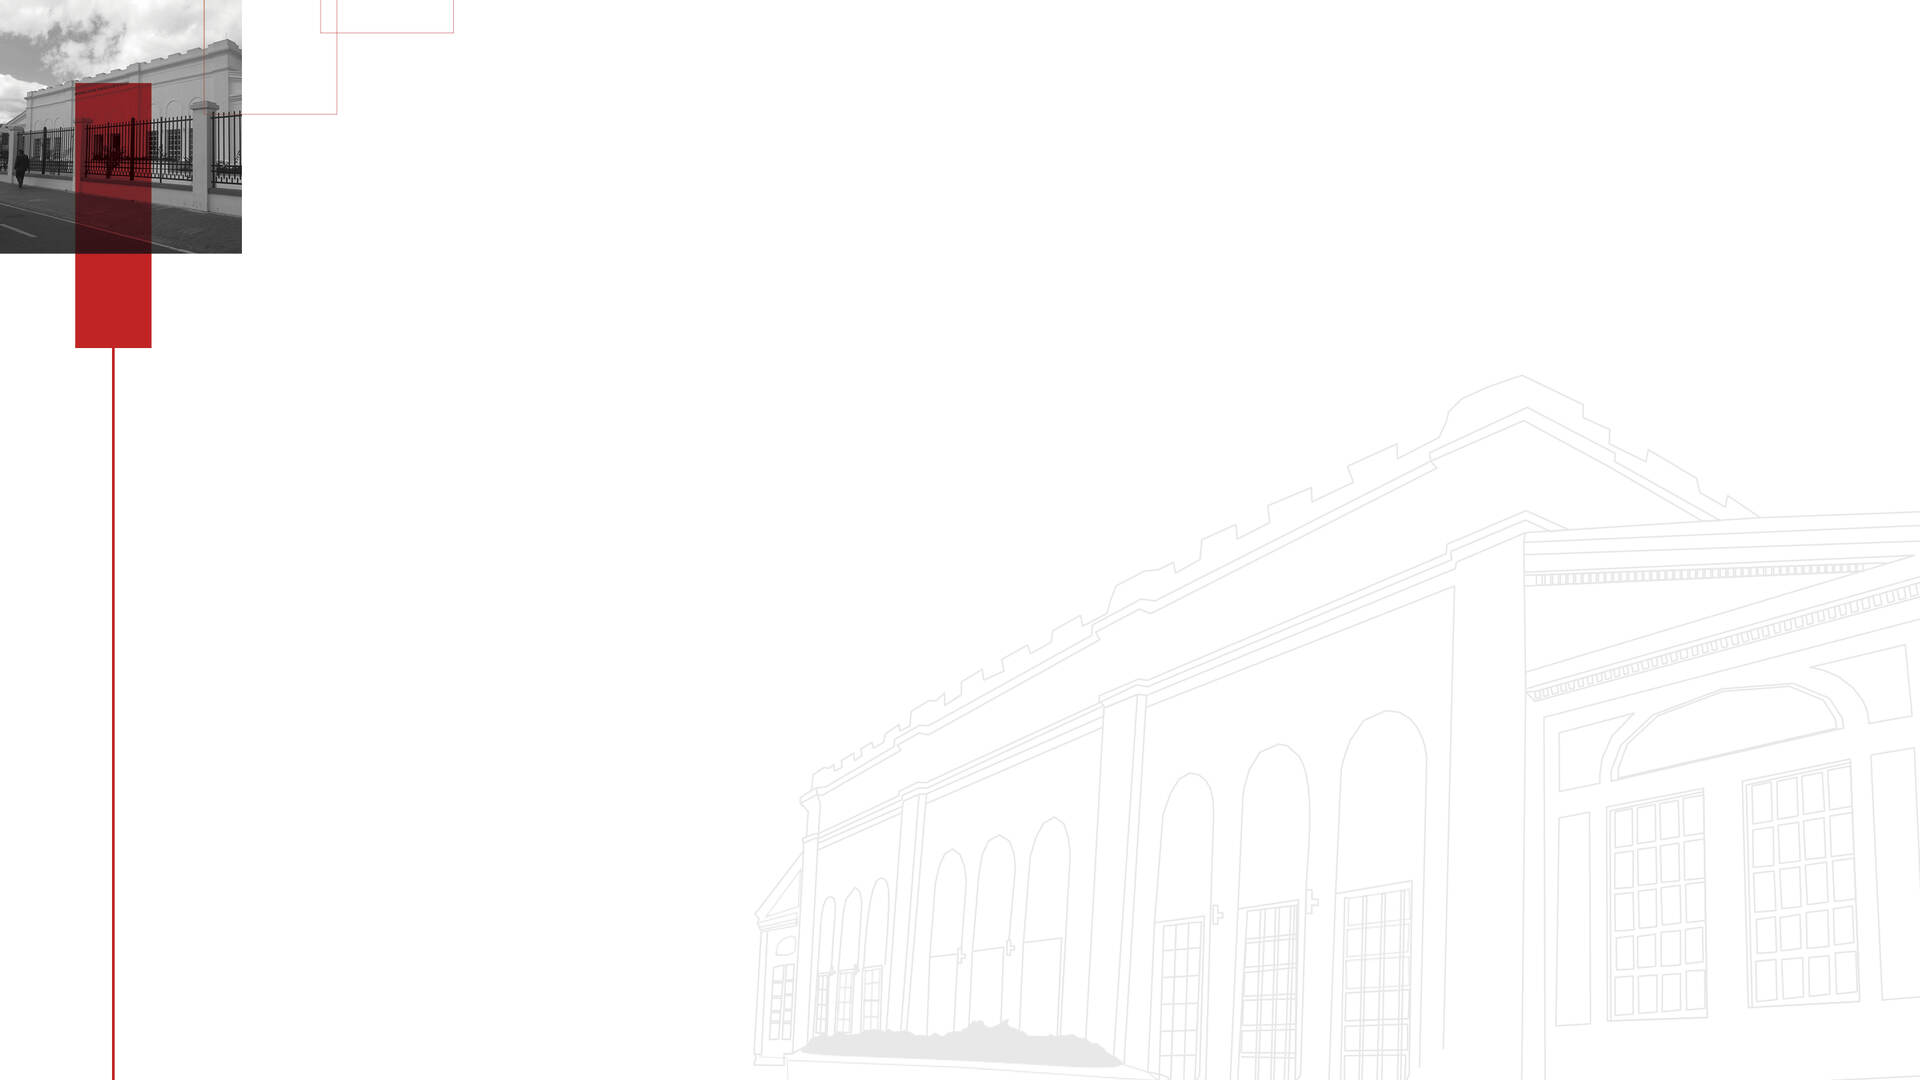
\includegraphics[width=\paperwidth,height=\paperheight]{assets/fondo_contenido.jpg}
}

% Estilos TikZ para diagramas de flujo
\tikzset{
  fcBase/.style={
    font=\fontsize{6.5pt}{7.5pt}\selectfont,
    text centered,
    inner sep=3pt,
    line width=0.6pt,
    draw=UDBorder,
    rounded corners=2.5pt
  },
  fcStart/.style={
    fcBase,
    fill=UDBlue!12,
    draw=UDBlue,
    text=UDSable,
    minimum height=0.55cm
  },
  fcStep/.style={
    fcBase,
    fill=white,
    draw=UDSilver,
    text=UDSable,
    minimum height=0.52cm
  },
  fcConv/.style={
    fcBase,
    fill=UDRed!10,
    draw=UDRed,
    text=UDSable,
    minimum height=0.52cm
  },
  fcRelu/.style={
    fcBase,
    fill=UDGold!15,
    draw=UDGold,
    text=UDSable,
    minimum height=0.52cm
  },
  fcPool/.style={
    fcBase,
    fill=UDGreen!12,
    draw=UDDarkGreen,
    text=UDSable,
    minimum height=0.52cm
  },
  fcDecision/.style={
    diamond,
    aspect=2.8,
    fcBase,
    fill=UDGold!20,
    draw=UDGold!90!black,
    text=UDSable,
    inner sep=2pt
  },
  fcArrow/.style={
    thick,
    color=UDRed,
    -{Latex[length=2mm]}
  },
  fcArrowBlue/.style={
    thick,
    color=UDBlue,
    -{Latex[length=2mm]}
  },
  fcArrowGreen/.style={
    thick,
    color=UDDarkGreen,
    -{Latex[length=2mm]}
  }
}

% Entorno de tarjeta personalizada
\newcommand{\UDCard}[3]{%
  \begin{tikzpicture}
    \node[fill=#1, draw=#2, rounded corners=3pt, line width=0.7pt, inner sep=5pt, text width=0.96\linewidth] {
      #3
    };
  \end{tikzpicture}
}

\begin{document}

% ------------------------------------------------------------------------------
% DIAPOSITIVA 1: PORTADA
% ------------------------------------------------------------------------------
{
\setbeamertemplate{background}{}
\begin{frame}[plain]
  \begin{tikzpicture}[remember picture,overlay]
    \node[anchor=south west,inner sep=0pt] at (current page.south west) {%
      
\includegraphics[width=\paperwidth,height=\paperheight]{assets/portada_base.jpg}%
    };

    % Panel de texto centrado con alta legibilidad
    \node[anchor=north west, align=left, inner sep=0pt]
      at ([xshift=8.10cm, yshift=-2.60cm]current page.north west) {
        \begin{minipage}{5.5cm}
          {\cambriafont\fontsize{13pt}{15.5pt}\bfseries\color{UDSable}CNN en OpenACC\par}
          \vspace{0.06cm}
          {\cambriafont\fontsize{8.2pt}{10pt}\bfseries\color{UDRed} Convolución 2D + ReLU + MaxPooling 2D\par}
          \vspace{0.08cm}
          {\color{UDRed}\rule{5.0cm}{1.0pt}\par}
          \vspace{0.10cm}
          {\cambriafont\fontsize{8.2pt}{9.8pt}\bfseries\color{UDSable} Juan Felipe Rodríguez \quad \textnormal{\color{UDSilver}|} \quad \textnormal{\color{UDSable}MCIC}\par}
          \vspace{0.04cm}
          {\fontsize{6.8pt}{8.2pt}\color{UDSable} Maestría en Ciencias de la\\ Información y las Comunicaciones\par}
          \vspace{0.04cm}
          {\fontsize{6.4pt}{7.6pt}\color{UDBlue} Computación Paralela y Distribuida \\ 2026\par}
        \end{minipage}
      };
  \end{tikzpicture}
\end{frame}
}

% ------------------------------------------------------------------------------
% DIAPOSITIVA 2: FLUJOGRAMA GENERAL DE LA TUBERÍA (HORIZONTAL COMPACTO)
% ------------------------------------------------------------------------------
\begin{frame}{Flujograma General de la Tubería y Memoria}{Ciclo de vida Host-Device y persistencia en VRAM con OpenACC}
  \vspace{-0.15cm}

  % Diagrama horizontal de flujo Host -> GPU -> Host
  \begin{center}
  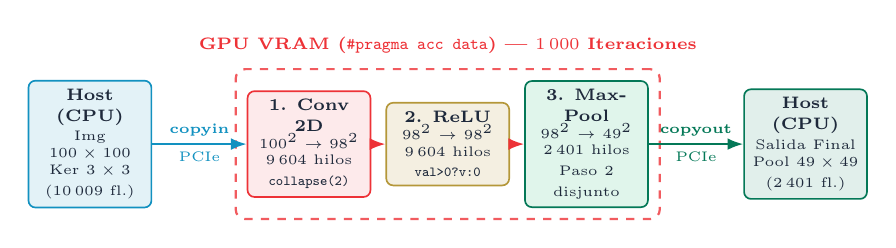
\begin{tikzpicture}[auto]
    % Etapas GPU centrales
    \node (s1) [fcConv, text width=1.35cm, minimum height=1.05cm] {
      \textbf{1. Conv 2D}\\
      \fontsize{5.0pt}{6.0pt}\selectfont
      $100^2 \rightarrow 98^2$\\
      $9\,604$ hilos\\
      \texttt{collapse(2)}
    };

    \node (s2) [fcRelu, right=0.18cm of s1, text width=1.35cm, minimum height=1.05cm] {
      \textbf{2. ReLU}\\
      \fontsize{5.0pt}{6.0pt}\selectfont
      $98^2 \rightarrow 98^2$\\
      $9\,604$ hilos\\
      \texttt{val>0?v:0}
    };

    \node (s3) [fcPool, right=0.18cm of s2, text width=1.35cm, minimum height=1.05cm] {
      \textbf{3. MaxPool}\\
      \fontsize{5.0pt}{6.0pt}\selectfont
      $98^2 \rightarrow 49^2$\\
      $2\,401$ hilos\\
      Paso 2 disjunto
    };

    \draw [fcArrow] (s1) -- (s2);
    \draw [fcArrow] (s2) -- (s3);

    % Caja GPU delimitadora y etiqueta
    \node (gpu_box) [draw=UDRed!80, rounded corners=3.5pt, dashed, line width=0.8pt, inner sep=4pt, fit=(s1) (s2) (s3)] {};
    \node (gpu_label) [above=0.06cm of gpu_box.north, font=\fontsize{6.0pt}{7.0pt}\selectfont\bfseries, text=UDRed] {
      GPU VRAM (\texttt{\#pragma acc data}) --- $1\,000$ Iteraciones
    };

    % Host In (a la izquierda)
    \node (host_in) [fcStart, left=1.20cm of s1, text width=1.35cm, minimum height=1.05cm] {
      \textbf{Host (CPU)}\\[0.03cm]
      \fontsize{5.2pt}{6.2pt}\selectfont
      Img $100 \times 100$\\
      Ker $3 \times 3$\\
      ($10\,009$ fl.)
    };

    % Host Out (a la derecha)
    \node (host_out) [fcStart, right=1.20cm of s3, fill=UDDarkGreen!12, draw=UDDarkGreen, text width=1.35cm, minimum height=1.05cm] {
      \textbf{Host (CPU)}\\[0.03cm]
      \fontsize{5.2pt}{6.2pt}\selectfont
      Salida Final\\
      Pool $49 \times 49$\\
      ($2\,401$ fl.)
    };

    % Flechas PCIe perfectamente horizontales
    \draw [fcArrowBlue] (host_in) -- 
      node[above, font=\fontsize{5.4pt}{6.4pt}\selectfont\bfseries, text=UDBlue, yshift=-1pt] {copyin}
      node[below, font=\fontsize{4.8pt}{5.8pt}\selectfont, text=UDBlue, yshift=1pt] {PCIe} (s1);

    \draw [fcArrowGreen] (s3) -- 
      node[above, font=\fontsize{5.4pt}{6.4pt}\selectfont\bfseries, text=UDDarkGreen, yshift=-1pt] {copyout}
      node[below, font=\fontsize{4.8pt}{5.8pt}\selectfont, text=UDDarkGreen, yshift=1pt] {PCIe} (host_out);
  \end{tikzpicture}
  \end{center}

  \vspace{0.15cm}

  % 3 Tarjetas de principios de diseño
  \begin{columns}[T]
    \begin{column}{0.32\textwidth}
      \UDCard{white}{UDBorder}{
        \textbf{\color{UDBlue}1. Transferencias PCIe:}
        \vspace{0.06cm}
        {\fontsize{6.8pt}{8.2pt}\selectfont
        \texttt{copyin} y \texttt{copyout} operan una sola vez al inicio y al final de la ráfaga completa.}
      }
    \end{column}
    \begin{column}{0.32\textwidth}
      \UDCard{white}{UDBorder}{
        \textbf{\color{UDRed}2. Encadenamiento VRAM:}
        \vspace{0.06cm}
        {\fontsize{6.8pt}{8.2pt}\selectfont
        Buffers \texttt{conv} y \texttt{relu} asignados con \texttt{create} con \textbf{cero tráfico PCIe} intermedio.}
      }
    \end{column}
    \begin{column}{0.32\textwidth}
      \UDCard{white}{UDBorder}{
        \textbf{\color{UDDarkGreen}3. Coalescencia 1D:}
        \vspace{0.06cm}
        {\fontsize{6.8pt}{8.2pt}\selectfont
        Arreglos continuos 1D (\texttt{i*W + j}) para accesos óptimos en memoria global GPU.}
      }
    \end{column}
  \end{columns}
\end{frame}

% ------------------------------------------------------------------------------
% DIAPOSITIVA 3: FLUJOGRAMA ETAPA 1 - CONVOLUCIÓN 2D
% ------------------------------------------------------------------------------
\begin{frame}{Etapa 1: Convolución 2D (Flujograma y Paralelismo)}{Filtrado espacial $3 \times 3$ colapsado en $9\,604$ hilos paralelos}
  \vspace{-0.15cm}
  \begin{columns}[T]
    % Flujograma de la etapa
    \begin{column}{0.50\textwidth}
      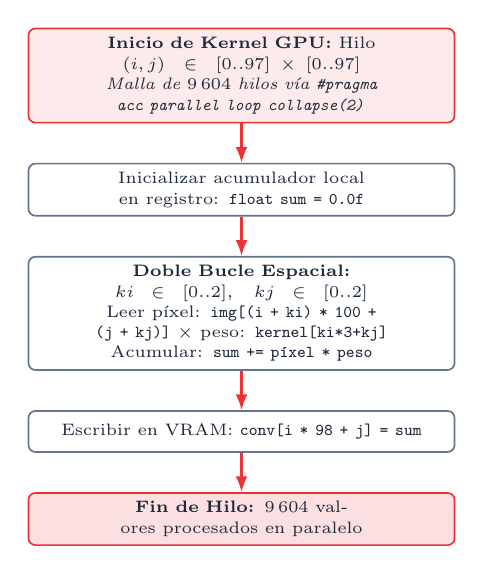
\begin{tikzpicture}[node distance=0.50cm, auto]
        \node (e1) [fcConv, text width=5.2cm] {
          \textbf{Inicio de Kernel GPU:} Hilo $(i, j) \in [0..97] \times [0..97]$\\
          \textit{Malla de $9\,604$ hilos vía \texttt{\#pragma acc parallel loop collapse(2)}}
        };
        \node (e2) [fcStep, below=of e1, text width=5.2cm] {
          Inicializar acumulador local en registro: \texttt{float sum = 0.0f}
        };
        \node (e3) [fcStep, below=of e2, text width=5.2cm] {
          \textbf{Doble Bucle Espacial:} $ki \in [0..2], \; kj \in [0..2]$\\
          \fontsize{6.2pt}{7.2pt}\selectfont
          Leer píxel: \texttt{img[(i + ki) * 100 + (j + kj)]} $\times$ peso: \texttt{kernel[ki*3+kj]}\\
          Acumular: \texttt{sum += píxel * peso}
        };
        \node (e4) [fcStep, below=of e3, text width=5.2cm] {
          Escribir en VRAM: \texttt{conv[i * 98 + j] = sum}
        };
        \node (e5) [fcConv, below=of e4, text width=5.2cm, fill=UDRed!15] {
          \textbf{Fin de Hilo:} $9\,604$ valores procesados en paralelo
        };

        \draw [fcArrow] (e1) -- (e2);
        \draw [fcArrow] (e2) -- (e3);
        \draw [fcArrow] (e3) -- (e4);
        \draw [fcArrow] (e4) -- (e5);
      \end{tikzpicture}
    \end{column}

    % Explicación técnica y código
    \begin{column}{0.48\textwidth}
      \UDCard{white}{UDBorder}{
        \textbf{\color{UDRed}Operación Aritmética:}
        \vspace{0.08cm}
        \begin{itemize}\setlength{\itemsep}{0.1cm}\fontsize{7pt}{8.5pt}\selectfont
          \item \textbf{Carga local:} $9$ productos y $9$ acumulaciones ($18$ FLOPs/píxel).
          \item \textbf{Total etapa:} $9\,604 \times 18 \approx 172.8$ kFLOPs/iteración.
          \item \textbf{Colapso 2D:} Fusión bidimensional que evita subutilizar la GPU ($98 \rightarrow 9\,604$ hilos).
        \end{itemize}
      }
      \vspace{0.12cm}
      \UDCard{UDLightGray}{UDRed!60}{
        \fontsize{6.3pt}{7.6pt}\selectfont\ttfamily
        \textcolor{UDRed}{\#pragma acc parallel loop collapse(2)}\\
        for (int i = 0; i < 98; ++i) \{\\
        \hspace*{0.2cm}for (int j = 0; j < 98; ++j) \{\\
        \hspace*{0.4cm}float sum = 0.0f;\\
        \hspace*{0.4cm}for (int ki = 0; ki < 3; ++ki)\\
        \hspace*{0.6cm}for (int kj = 0; kj < 3; ++kj)\\
        \hspace*{0.8cm}sum += img[...] * kernel[...];\\
        \hspace*{0.4cm}conv[i * 98 + j] = sum;\\
        \hspace*{0.2cm}\}\\
        \}
      }
    \end{column}
  \end{columns}
\end{frame}

% ------------------------------------------------------------------------------
% DIAPOSITIVA 4: FLUJOGRAMA ETAPA 2 - ACTIVACIÓN RELU
% ------------------------------------------------------------------------------
\begin{frame}{Etapa 2: Activación ReLU (Flujograma y Evaluación)}{Truncamiento no lineal sin dependencias espaciales}
  \vspace{-0.15cm}
  \begin{columns}[T]
    % Flujograma
    \begin{column}{0.50\textwidth}
      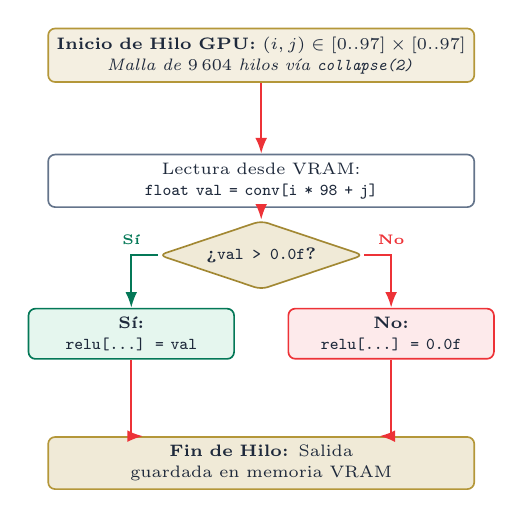
\begin{tikzpicture}[node distance=0.90cm, auto]
        \node (r1) [fcRelu, text width=5.2cm] {
          \textbf{Inicio de Hilo GPU:} $(i, j) \in [0..97] \times [0..97]$\\
          \textit{Malla de $9\,604$ hilos vía \texttt{collapse(2)}}
        };
        \node (r2) [fcStep, below=of r1, text width=5.2cm] {
          Lectura desde VRAM: \texttt{float val = conv[i * 98 + j]}
        };
        \node (r3) [fcDecision, below=0.15cm of r2, minimum width=2.6cm, minimum height=0.6cm] {
          \textbf{¿\texttt{val > 0.0f}?}
        };
        \node (r4_yes) [fcStep, below=0.22cm of r3, xshift=-1.65cm, text width=2.4cm, fill=UDGreen!10, draw=UDDarkGreen] {
          \textbf{Sí:}\\
          \texttt{relu[...] = val}
        };
        \node (r4_no) [fcStep, below=0.22cm of r3, xshift=1.65cm, text width=2.4cm, fill=UDRed!10, draw=UDRed] {
          \textbf{No:}\\
          \texttt{relu[...] = 0.0f}
        };
        \node (r5) [fcRelu, below=1.85cm of r3, text width=5.2cm, fill=UDGold!20] {
          \textbf{Fin de Hilo:} Salida guardada en memoria VRAM
        };

        \draw [fcArrow] (r1) -- (r2);
        \draw [fcArrow] (r2) -- (r3);
        \draw [fcArrowGreen] (r3) -| node[above, font=\tiny\bfseries, text=UDDarkGreen] {Sí} (r4_yes);
        \draw [fcArrow] (r3) -| node[above, font=\tiny\bfseries, text=UDRed] {No} (r4_no);
        \draw [fcArrow] (r4_yes.south) |- ([xshift=-1.5cm]r5.north);
        \draw [fcArrow] (r4_no.south) |- ([xshift=1.5cm]r5.north);
      \end{tikzpicture}
    \end{column}

    % Explicación técnica y código
    \begin{column}{0.48\textwidth}
      \UDCard{white}{UDBorder}{
        \textbf{\color{UDGold!90!black}Fundamentos de Activación:}
        \vspace{0.08cm}
        \begin{itemize}\setlength{\itemsep}{0.1cm}\fontsize{7pt}{8.5pt}\selectfont
          \item \textbf{Sin dependencias:} Operación puramente local e independiente elemento a elemento.
          \item \textbf{Preservación dimensional:} Entrada y salida idénticas de $98 \times 98$ ($9\,604$ elementos).
          \item \textbf{Cero transferencias:} Consume \texttt{conv} en VRAM y produce \texttt{relu} en VRAM.
        \end{itemize}
      }
      \vspace{0.12cm}
      \UDCard{UDLightGray}{UDGold!80}{
        \fontsize{5.8pt}{7.0pt}\selectfont\ttfamily
        \textcolor{UDRed}{\#pragma acc parallel loop collapse(2)}\\
        for (int i = 0; i < 98; ++i) \{\\
        \hspace*{0.2cm}for (int j = 0; j < 98; ++j) \{\\
        \hspace*{0.4cm}float val = conv[i * 98 + j];\\
        \hspace*{0.4cm}relu[i * 98 + j] = (val > 0.0f) ? val : 0.0f;\\
        \hspace*{0.2cm}\}\\
        \}
      }
    \end{column}
  \end{columns}
\end{frame}

% ------------------------------------------------------------------------------
% DIAPOSITIVA 5: FLUJOGRAMA ETAPA 3 - MAXPOOLING 2D
% ------------------------------------------------------------------------------
\begin{frame}{Etapa 3: MaxPooling 2D (Flujograma y Reducción)}{Submuestreo disjunto con paso 2 sin parámetros entrenables}
  \vspace{-0.15cm}
  \begin{columns}[T]
    % Flujograma
    \begin{column}{0.50\textwidth}
      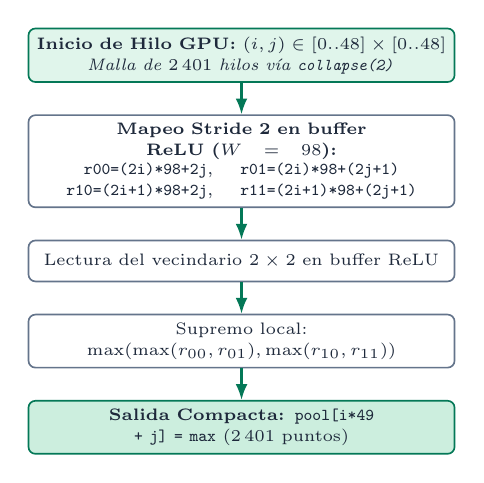
\begin{tikzpicture}[node distance=0.4cm, auto]
        \node (p1) [fcPool, text width=5.2cm] {
          \textbf{Inicio de Hilo GPU:} $(i, j) \in [0..48] \times [0..48]$\\
          \textit{Malla de $2\,401$ hilos vía \texttt{collapse(2)}}
        };
        \node (p2) [fcStep, below=of p1, text width=5.2cm] {
          \textbf{Mapeo Stride 2 en buffer ReLU ($W=98$):}\\
          \fontsize{5.8pt}{6.8pt}\selectfont
          \texttt{r00=(2i)*98+2j}, \quad \texttt{r01=(2i)*98+(2j+1)}\\
          \texttt{r10=(2i+1)*98+2j}, \quad \texttt{r11=(2i+1)*98+(2j+1)}
        };
        \node (p3) [fcStep, below=of p2, text width=5.2cm] {
          Lectura del vecindario $2\times 2$ en buffer ReLU
        };
        \node (p4) [fcStep, below=of p3, text width=5.2cm] {
          Supremo local: $\max(\max(r_{00}, r_{01}), \max(r_{10}, r_{11}))$
        };
        \node (p5) [fcPool, below=of p4, text width=5.2cm, fill=UDGreen!20] {
          \textbf{Salida Compacta:} \texttt{pool[i*49 + j] = max} ($2\,401$ puntos)
        };

        \draw [fcArrowGreen] (p1) -- (p2);
        \draw [fcArrowGreen] (p2) -- (p3);
        \draw [fcArrowGreen] (p3) -- (p4);
        \draw [fcArrowGreen] (p4) -- (p5);
      \end{tikzpicture}
    \end{column}

    % Corrección teórica y código
    \begin{column}{0.48\textwidth}
      \UDCard{UDRed!6}{UDRed}{
        \textbf{\color{UDRed}Corrección Teórica (Ventana 2x2):}
        \vspace{0.06cm}
        \begin{itemize}\setlength{\itemsep}{0.06cm}\fontsize{6.8pt}{8.0pt}\selectfont
          \item La ``ventana 2x2'' \textbf{no es una matriz} ni posee pesos numéricos entrenables.
          \item Es únicamente un \textbf{rango de lectura espacial}: extrae el supremo de las 4 celdas continuas.
        \end{itemize}
      }
      \vspace{0.08cm}
      \UDCard{UDLightGray}{UDDarkGreen!80}{
        \fontsize{5.6pt}{6.8pt}\selectfont\ttfamily
        \textcolor{UDRed}{\#pragma acc parallel loop collapse(2)}\\
        for (int i = 0; i < 49; ++i) \{\\
        \hspace*{0.15cm}for (int j = 0; j < 49; ++j) \{\\
        \hspace*{0.3cm}int r0 = (2*i)*98 + 2*j, r1 = (2*i+1)*98 + 2*j;\\
        \hspace*{0.3cm}float m0 = std::max(relu[r0], relu[r0 + 1]);\\
        \hspace*{0.3cm}float m1 = std::max(relu[r1], relu[r1 + 1]);\\
        \hspace*{0.3cm}pool[i*49 + j] = std::max(m0, m1);\\
        \hspace*{0.15cm}\}\\
        \}
      }
    \end{column}
  \end{columns}
\end{frame}

% ------------------------------------------------------------------------------
% DIAPOSITIVA 6: ESTRATEGIA DE DATOS EN OPENACC
% ------------------------------------------------------------------------------
\begin{frame}{Estrategia de Memoria en GPU con OpenACC}{Eliminación de transferencias intermedias en el bus PCIe}
  \vspace{-0.15cm}
  \begin{columns}[T]
    \begin{column}{0.53\textwidth}
      \UDCard{UDLightGray}{UDBlue!80}{
        \fontsize{6.8pt}{8.2pt}\selectfont\ttfamily
        \textcolor{UDRed}{\#pragma acc data} \textbackslash\\
        \hspace*{0.35cm}\textcolor{UDBlue}{copyin}(img[0:10000], kernel[0:9]) \textbackslash\\
        \hspace*{0.35cm}\textcolor{UDGreen}{create}(conv[0:9604], relu[0:9604]) \textbackslash\\
        \hspace*{0.35cm}\textcolor{UDRed}{copyout}(pool[0:2401])\\
        \{\\
        \hspace*{0.35cm}for (int it = 0; it < 1000; ++it) \{\\
        \hspace*{0.7cm}// 1. Convolucion 2D (GPU)\\
        \hspace*{0.7cm}// 2. Activacion ReLU (GPU)\\
        \hspace*{0.7cm}// 3. MaxPooling 2D  (GPU)\\
        \hspace*{0.35cm}\}\\
        \}
      }
    \end{column}

    \begin{column}{0.45\textwidth}
      \UDCard{white}{UDBorder}{
        \textbf{\color{UDSable}Análisis de Cláusulas de Datos:}
        \vspace{0.12cm}
        \begin{itemize}\setlength{\itemsep}{0.16cm}\fontsize{7.2pt}{9pt}\selectfont
          \item \textbf{\color{UDBlue}copyin:} Transfiere la imagen y el kernel a la GPU \textbf{una sola vez} al inicio.
          \item \textbf{\color{UDGreen}create:} Asigna buffers temporales en VRAM. \textbf{Cero transferencias PCIe} durante las 1,000 repeticiones.
          \item \textbf{\color{UDRed}copyout:} Retorna únicamente la salida compacta ($49 \times 49$) al Host al culminar la ráfaga.
        \end{itemize}
      }
    \end{column}
  \end{columns}
\end{frame}

% ------------------------------------------------------------------------------
% DIAPOSITIVA 7: RESULTADOS EXPERIMENTALES Y LEY DE AMDAHL
% ------------------------------------------------------------------------------
\begin{frame}{Resultados Experimentales y Ley de Amdahl}{Aceleración neta de cómputo ($15.45\times$) y total de sistema ($13.08\times$)}
  \vspace{-0.15cm}
  \begin{columns}[T]
    \begin{column}{0.51\textwidth}
      \UDCard{white}{UDBorder}{
        \textbf{\color{UDSable}Rendimiento ($1\,000$ Iteraciones):}
        \vspace{0.08cm}
        {\fontsize{6.6pt}{8.0pt}\selectfont
        \setlength{\tabcolsep}{2.5pt}
        \begin{tabular}{@{}llr@{}}
          \toprule
          \textbf{Métrica de Evaluación} & \textbf{Valor} & \textbf{Unidad} \\
          \midrule
          CPU Secuencial ($T_{\text{CPU}}$) & $32.46$ & ms \\
          GPU Cómputo Neto ($T_{\text{Kernel}}$) & $2.10$ & ms \\
          GPU Total con E/S ($T_{\text{Total}}$) & $2.48$ & ms \\
          Overhead de bus PCIe & $0.38$ & ms ($15.3\%$) \\
          \midrule
          \textbf{Speedup Cómputo ($S_{\text{cómputo}}$)} & \textbf{15.45x} & Aceleración \\
          \textbf{Speedup Total ($S_{\text{total}}$)} & \textbf{13.08x} & Aceleración \\
          \bottomrule
        \end{tabular}
        }
      }
      \vspace{0.08cm}
      \UDCard{UDGreen!8}{UDDarkGreen!70}{
        \fontsize{6.2pt}{7.4pt}\selectfont
        \textbf{\color{UDDarkGreen}Consistencia:} Verificación bit a bit exacta ($\Delta_{\max} = 0.000$).
      }
    \end{column}

    \begin{column}{0.47\textwidth}
      \UDCard{white}{UDBorder}{
        \textbf{\color{UDSable}Análisis con la Ley de Amdahl:}
        \vspace{0.12cm}
        \begin{itemize}\setlength{\itemsep}{0.16cm}\fontsize{7.2pt}{9pt}\selectfont
          \item \textbf{Granularidad de $100 \times 100$:} Carga moderada donde el costo de lanzamiento de kernels es perceptible.
          \item \textbf{Amortización del Bucle:} Con $N=1$, el bus PCIe dominaría arrojando $S < 1\times$. Con $N=1\,000$, el costo se amortiza a $0.38\ \mu\text{s}$/iteración.
          \item \textbf{Escalabilidad:} Matrices mayores ($1024 \times 1024$) saturan completamente los multiprocesadores CUDA.
        \end{itemize}
      }
    \end{column}
  \end{columns}
\end{frame}

% ------------------------------------------------------------------------------
% DIAPOSITIVA 8: CONCLUSIONES Y PRÓXIMOS PASOS
% ------------------------------------------------------------------------------
\begin{frame}{Conclusiones y Trabajo Futuro}{Lecciones aprendidas en HPC y próximos pasos}
  \vspace{-0.15cm}
  \begin{columns}[T]
    \begin{column}{0.48\textwidth}
      \UDCard{UDLightGray}{UDBlue!60}{
        \textbf{\color{UDBlue}Conclusiones Principales:}
        \vspace{0.12cm}
        \begin{itemize}\setlength{\itemsep}{0.16cm}\fontsize{7.3pt}{9.2pt}\selectfont
          \item \textbf{Aceleración Masiva:} OpenACC permitió superar en más de \textbf{$13\times$} a la CPU con directivas directas y portables.
          \item \textbf{Gestión de Datos:} El uso de \texttt{acc data} con \texttt{create} es el factor decisivo para evitar transferencias en el bus PCIe.
          \item \textbf{Colapso 2D:} La cláusula \texttt{collapse(2)} es indispensable para crear mallas de alta ocupación ($9\,604$ hilos).
        \end{itemize}
      }
    \end{column}

    \begin{column}{0.48\textwidth}
      \UDCard{UDLightGray}{UDGold!80}{
        \textbf{\color{UDGold!90!black}Trabajo Futuro:}
        \vspace{0.12cm}
        \begin{itemize}\setlength{\itemsep}{0.16cm}\fontsize{7.3pt}{9.2pt}\selectfont
          \item \textbf{Fusión de Kernels:} Integrar Convolución y ReLU en un solo kernel para procesar en registros y ahorrar accesos a VRAM.
          \item \textbf{Soporte Multicanal:} Extender la tubería a tensores 4D (batch, canales, alto, ancho) de modelos profundos (ResNet, VGG).
          \item \textbf{Memoria Compartida:} Aplicar directivas \texttt{cache} para reusar píxeles adyacentes en la convolución.
        \end{itemize}
      }
    \end{column}
  \end{columns}
\end{frame}

% ------------------------------------------------------------------------------
% DIAPOSITIVA 9: CIERRE INSTITUCIONAL
% ------------------------------------------------------------------------------
{
\setbeamertemplate{background}{}
\begin{frame}[plain]
  \begin{tikzpicture}[remember picture,overlay]
    \node[anchor=south west,inner sep=0pt] at (current page.south west) {%
      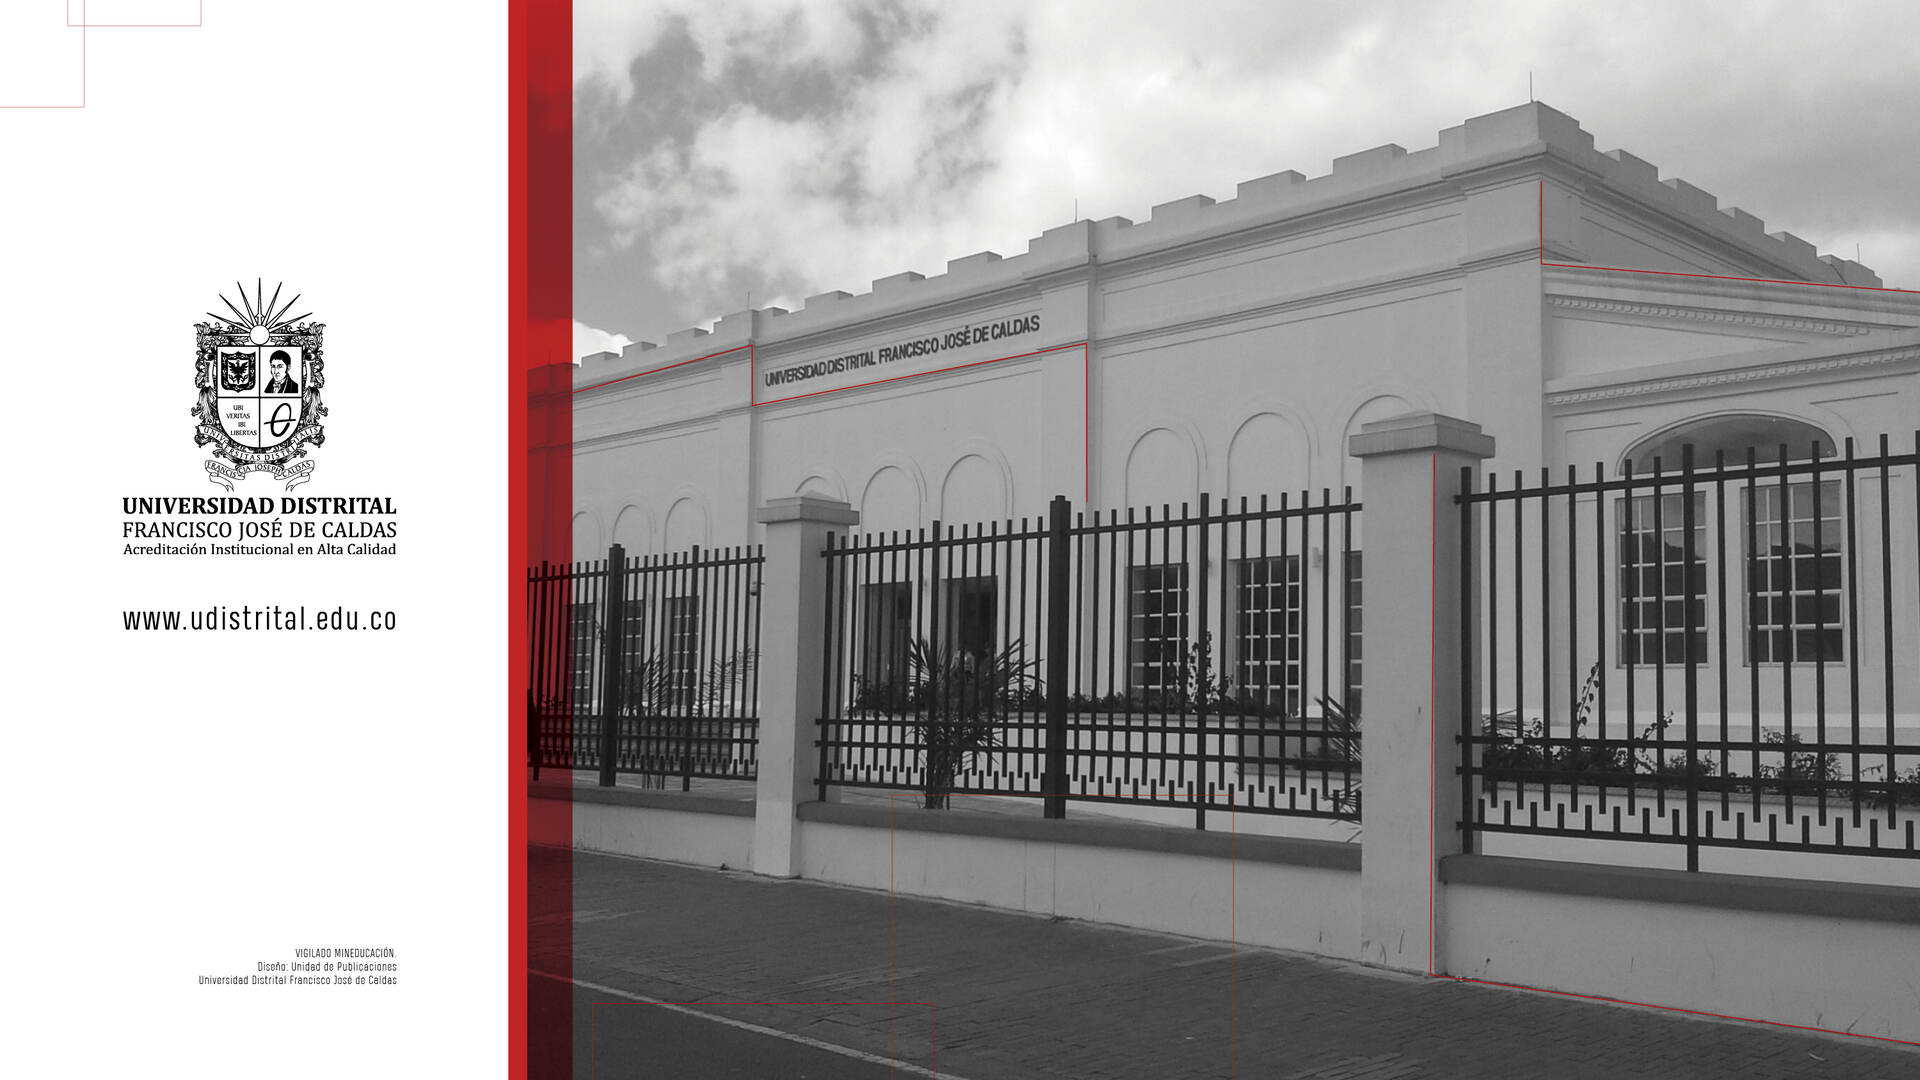
\includegraphics[width=\paperwidth,height=\paperheight]{assets/cierre_base.jpg}%
    };

    % Tarjeta elegante en el área derecha con datos de sustentación
    \node[anchor=center, fill=white, fill opacity=0.94, text opacity=1, rounded corners=4pt, inner sep=14pt, line width=0.8pt, draw=UDBorder] 
      at ([xshift=3.2cm, yshift=0.2cm]current page.center) {
        \begin{minipage}{5.8cm}
          \centering
          {\cambriafont\fontsize{16pt}{18pt}\bfseries\color{UDRed} ¡Muchas Gracias!\par}
          \vspace{0.25cm}
          {\cambriafont\fontsize{10.5pt}{13pt}\bfseries\color{UDSable} Espacio para Preguntas y Discusión\par}
          \vspace{0.25cm}
          {\color{UDRed}\rule{4.2cm}{1.2pt}\par}
          \vspace{0.25cm}
          {\cambriafont\fontsize{9pt}{11pt}\bfseries\color{UDSable} Juan Felipe Rodríguez\par}
          \vspace{0.08cm}
          {\fontsize{8pt}{10pt}\color{UDSable} Maestría en Ciencias de la Información\\y las Comunicaciones\par}
          \vspace{0.08cm}
          {\fontsize{7.5pt}{9pt}\color{UDSilver} Computación Paralela y Distribuida\par}
        \end{minipage}
      };
  \end{tikzpicture}
\end{frame}
}

\end{document}
